\documentclass[tikz,border=8pt]{standalone}
% Shared look for every TikZ diagram. Load with \input{../../tools/tikz-style.tex}
\usepackage[T1]{fontenc}
\usepackage{lmodern}
\renewcommand{\sfdefault}{lmr}  % diagrams use the same serif as the text
\usetikzlibrary{arrows.meta, positioning, shapes.geometric, calc, fit, backgrounds}
\definecolor{cblue}{HTML}{4C78A8}
\definecolor{corange}{HTML}{F58518}
\definecolor{cgreen}{HTML}{54A24B}
\definecolor{cred}{HTML}{E45756}
\definecolor{cpurple}{HTML}{B279A2}
\definecolor{cgrey}{HTML}{6B6B6B}
\tikzset{
  every picture/.style={font=\sffamily, line width=1.2pt},
  box/.style={draw=#1, fill=#1!12, rounded corners=4pt, align=center, inner sep=7pt, minimum height=1.1cm},
  box/.default=cgrey,
  arrow/.style={-{Stealth[length=3mm]}, draw=cgrey, line width=1.4pt},
  title/.style={font=\sffamily\bfseries\Large},
  note/.style={font=\sffamily\small, text=cgrey, align=center},
}
\AtBeginDocument{\hyphenpenalty=10000 \exhyphenpenalty=10000}

% The five sources of uncertainty (Thrun et al. 2005 ch.1, as listed in Khamis's L5 slides), each with one example.
\begin{document}
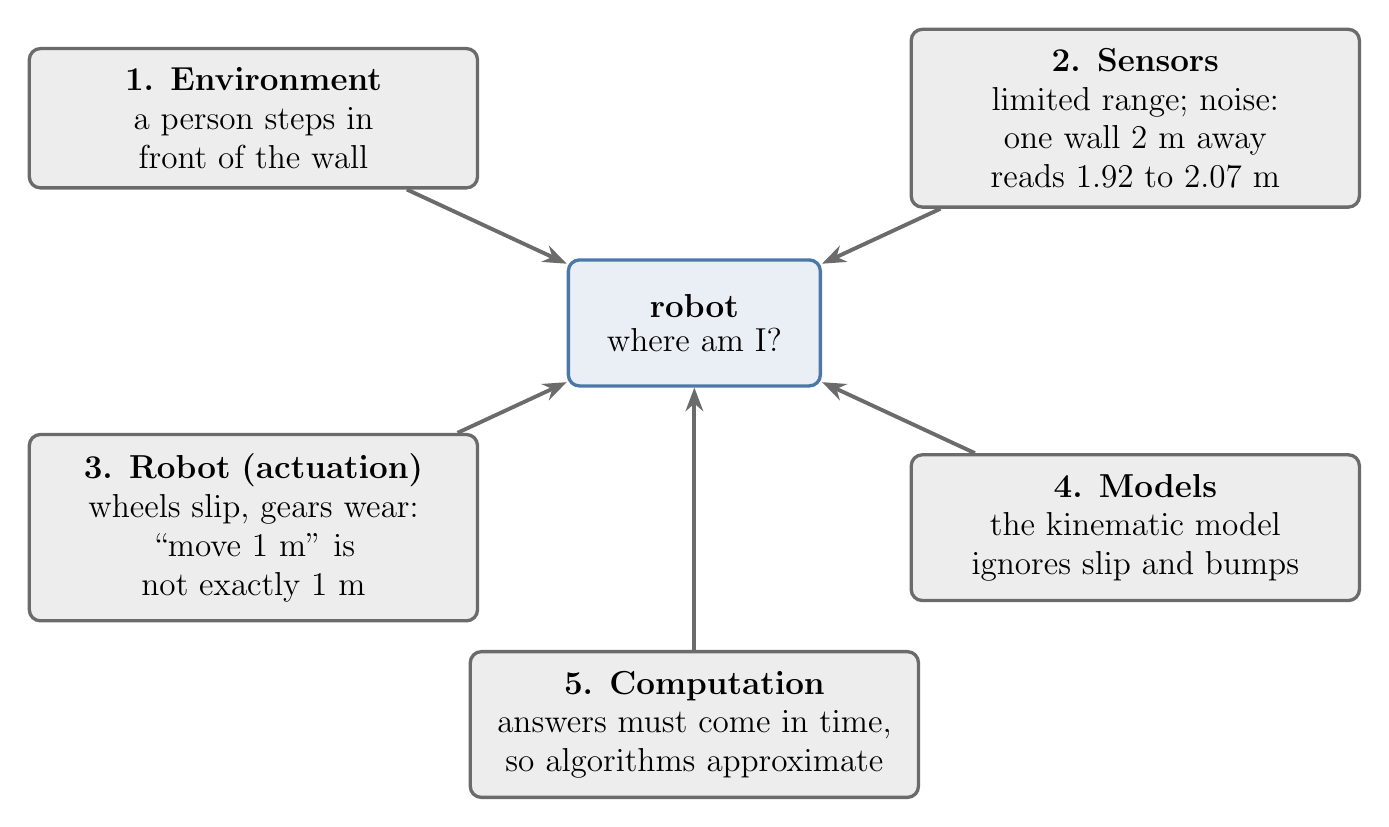
\begin{tikzpicture}[every node/.append style={font=\large}]
  \node[box=cblue, minimum width=3.2cm, minimum height=1.6cm] (r) at (0,0) {\textbf{robot}\\[-2pt]where am I?};
  \node[box=cgrey, text width=5.2cm] (e) at (-5.6,2.6) {\textbf{1. Environment}\\a person steps in front of the wall};
  \node[box=cgrey, text width=5.2cm] (s) at (5.6,2.6) {\textbf{2. Sensors}\\limited range; noise:\\one wall 2 m away\\reads 1.92 to 2.07 m};
  \node[box=cgrey, text width=5.2cm] (a) at (-5.6,-2.6) {\textbf{3. Robot (actuation)}\\wheels slip, gears wear:\\``move 1 m'' is not exactly 1 m};
  \node[box=cgrey, text width=5.2cm] (m) at (5.6,-2.6) {\textbf{4. Models}\\the kinematic model\\ignores slip and bumps};
  \node[box=cgrey, text width=5.2cm] (c) at (0,-5.1) {\textbf{5. Computation}\\answers must come in time,\\so algorithms approximate};
  \foreach \n in {e,s,a,m,c} \draw[arrow] (\n) -- (r);
\end{tikzpicture}
\end{document}
